\documentclass[12pt]{article}

\usepackage[paperwidth=40in,paperheight=30in,margin=0.55in]{geometry}
\usepackage[T1]{fontenc}
\usepackage{lmodern}
\usepackage{amsmath,amssymb}
\usepackage{graphicx}
\usepackage{xcolor}
\usepackage{tikz}
\usetikzlibrary{arrows.meta,calc,decorations.pathreplacing,positioning}
\usepackage{tcolorbox}
\usepackage{ragged2e}
\usepackage{microtype}
\usepackage{array}
\usepackage{helvet}
\renewcommand{\familydefault}{\sfdefault}

\definecolor{PosterBg}{HTML}{F4F6F8}
\definecolor{Navy}{HTML}{19324D}
\definecolor{Text}{HTML}{202124}
\definecolor{Muted}{HTML}{5F6368}
\definecolor{Border}{HTML}{D7DDE4}
\definecolor{SoftBlue}{HTML}{EAF3F8}
\definecolor{Blue}{HTML}{0072B2}
\definecolor{SoftRose}{HTML}{F7EDF2}
\definecolor{Rose}{HTML}{A64D79}
\definecolor{Charcoal}{HTML}{4D4D4D}
\definecolor{SoftGray}{HTML}{EEF1F4}

\pagecolor{PosterBg}
\color{Text}
\pagestyle{empty}
\setlength{\parindent}{0pt}
\setlength{\parskip}{0.13in}
\setlength{\fboxsep}{0pt}
\hyphenpenalty=10000
\exhyphenpenalty=10000

\newcommand{\BodyFont}{\fontsize{26}{31}\selectfont}
\newcommand{\SmallFont}{\fontsize{21}{25}\selectfont}
\newcommand{\TinyFont}{\fontsize{19}{23}\selectfont}
\newcommand{\ModeFont}{\fontsize{22}{26}\selectfont}
\newcommand{\QuestionFont}{\fontsize{32}{38}\selectfont}

\newtcolorbox{contentcard}[1][]{
  colback=white,
  colframe=Border,
  boxrule=1.2pt,
  arc=10pt,
  outer arc=10pt,
  left=0.30in,
  right=0.30in,
  top=0.26in,
  bottom=0.26in,
  before skip=0pt,
  after skip=0pt,
  before upper={\BodyFont\RaggedRight},
  #1
}

\newcommand{\sectionheading}[1]{%
  {\RaggedRight\color{Navy}\bfseries\fontsize{34}{39}\selectfont #1\par}%
  \vspace{0.05in}%
  {\color{Navy}\rule{0.78in}{3pt}}\par
  \vspace{0.12in}%
}

\newtcolorbox{questionbox}{
  colback=SoftBlue,
  colframe=Navy,
  boxrule=1.6pt,
  arc=8pt,
  left=0.24in,
  right=0.24in,
  top=0.18in,
  bottom=0.18in,
  before skip=0.16in,
  after skip=0.08in
}

% Single shared style for punchline statements: navy left bar, no full frame.
\newtcolorbox{insightbox}{
  colback=SoftGray,
  colframe=Navy,
  boxrule=0pt,
  leftrule=7pt,
  arc=2pt,
  left=0.24in,
  right=0.24in,
  top=0.16in,
  bottom=0.16in,
  before skip=0.13in,
  after skip=0.13in
}

\newtcolorbox{scopebox}{
  colback=SoftGray,
  colframe=Border,
  boxrule=1.0pt,
  arc=7pt,
  left=0.22in,
  right=0.22in,
  top=0.15in,
  bottom=0.15in,
  before skip=0.16in,
  after skip=0.08in
}

\newcommand{\metaitem}[2]{\textcolor{Navy}{\bfseries #1}\ #2}
\newcommand{\separator}{\hspace{0.25in}\textcolor{Border}{|}\hspace{0.25in}}
\newcommand{\takeawaynum}[1]{%
  \tikz[baseline=(n.base)]\node[circle,fill=Navy,text=white,font=\bfseries\fontsize{17}{18}\selectfont,inner sep=4.5pt] (n) {#1};%
}

\begin{document}
\BodyFont

% Header
\begin{tcolorbox}[
  colback=Navy,
  colframe=Navy,
  boxrule=0pt,
  arc=10pt,
  left=0.48in,
  right=0.48in,
  top=0.30in,
  bottom=0.28in,
  height=3.25in
]
\begin{minipage}[c][2.55in][c]{0.77\linewidth}
  {\color{white}\bfseries\fontsize{78}{84}\selectfont Attention Beyond the Training Length}\par
  \vspace{0.12in}
  {\color{white!88}\fontsize{31}{37}\selectfont
    How Score Scaling Controls Length Generalization in a Reduced Binary Attention Classifier}
\end{minipage}%
\hfill
\begin{minipage}[c][2.55in][c]{0.20\linewidth}
  \RaggedLeft
  {\color{white}\bfseries\fontsize{29}{34}\selectfont Aaron Shin}\par
  \vspace{0.10in}
  {\color{white!82}\fontsize{20}{25}\selectfont Deep Network Understanding Lab\\Dickinson College}
\end{minipage}
\end{tcolorbox}

\vspace{0.32in}

% Three reading regions built on a 1 + 2 + 1 column grid.
\noindent
\begin{minipage}[t]{9.30in}
\vspace{0pt}
\begin{contentcard}[height=5.35in]
\sectionheading{Motivation}
Training on short sequences does not guarantee reliable performance on much
longer inputs \textbf{[2]}. As sequence length grows, the target must compete
with more non-target tokens for the same attention budget.
\begin{questionbox}
\centering\QuestionFont\bfseries\color{Navy}
How must attention sharpen with length to remain concentrated on the target?
\end{questionbox}
\end{contentcard}

\vspace{0.28in}
\begin{contentcard}[height=19.17in]
\begin{minipage}[t][18.48in][t]{\linewidth}
\vspace{0pt}
\sectionheading{Why Fixed Attention Dilutes with Length}
The model detects whether a designated target token is present in the sequence.

\vfill
\begin{center}
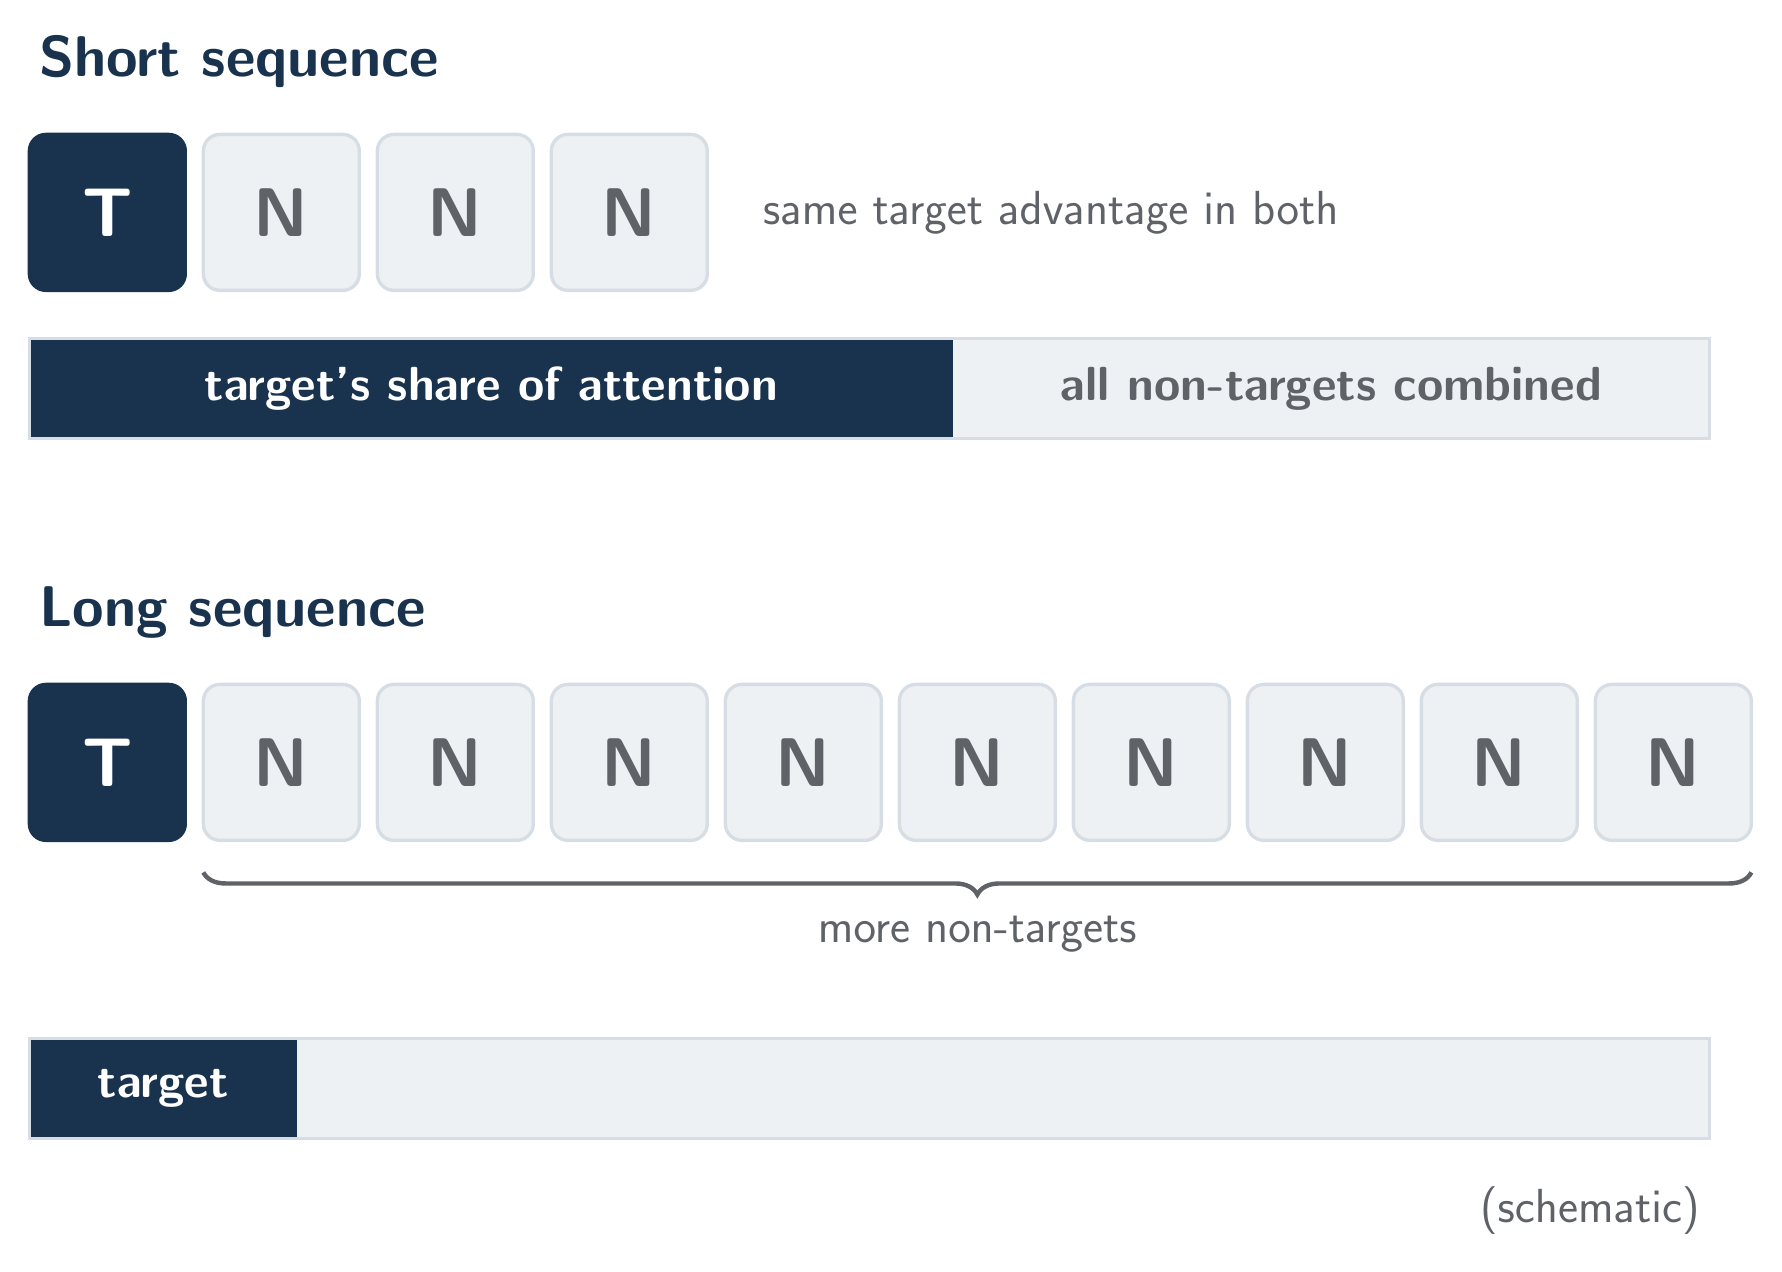
\begin{tikzpicture}[
  x=1in,
  y=1in,
  token/.style={minimum width=0.78in,minimum height=0.78in,rounded corners=6pt,draw=Border,line width=1.2pt,font=\bfseries\fontsize{26}{28}\selectfont,inner sep=0pt},
  non/.style={token,fill=SoftGray,text=Muted},
  target/.style={token,fill=Navy,text=white,draw=Navy},
  rowlabel/.style={font=\bfseries\fontsize{22}{26}\selectfont,text=Navy,anchor=west},
  note/.style={font=\fontsize{19}{23}\selectfont,text=Muted},
  barlabel/.style={font=\bfseries\fontsize{18}{21}\selectfont}
]
  % Short scene
  \node[rowlabel] at (0,8.30) {Short sequence};
  \node[target] at (0.39,7.55) {T};
  \foreach \i in {1,2,3} {\node[non] at (0.39+\i*0.87,7.55) {N};}
  \node[note,anchor=west] at (3.62,7.55) {same target advantage in both};
  \fill[Navy] (0,6.42) rectangle (4.62,6.92);
  \fill[SoftGray] (4.62,6.42) rectangle (8.40,6.92);
  \draw[Border,line width=1pt] (0,6.42) rectangle (8.40,6.92);
  \node[barlabel,text=white] at (2.31,6.67) {target's share of attention};
  \node[barlabel,text=Muted] at (6.51,6.67) {all non-targets combined};

  % Long scene
  \node[rowlabel] at (0,5.55) {Long sequence};
  \node[target] at (0.39,4.80) {T};
  \foreach \i in {1,...,9} {\node[non] at (0.39+\i*0.87,4.80) {N};}
  \draw[decorate,decoration={brace,mirror,amplitude=8pt},Muted,line width=1.6pt]
    (0.87,4.25) -- (8.61,4.25)
    node[midway,below=0.16in,note] {more non-targets};
  \fill[Navy] (0,2.92) rectangle (1.34,3.42);
  \fill[SoftGray] (1.34,2.92) rectangle (8.40,3.42);
  \draw[Border,line width=1pt] (0,2.92) rectangle (8.40,3.42);
  \node[barlabel,text=white] at (0.67,3.17) {\fontsize{16}{18}\selectfont target};
  \node[note,anchor=east] at (8.40,2.56) {(schematic)};
\end{tikzpicture}
\end{center}

\vfill
\begin{insightbox}
\textbf{A fixed score margin separates the target from each non-target, but
cannot offset their growing aggregate weight.}
\end{insightbox}

\vfill
\begin{tcolorbox}[colback=SoftGray,colframe=Border,boxrule=1pt,arc=6pt,left=0.20in,right=0.20in,top=0.17in,bottom=0.16in]
\SmallFont
Let $p_t(n)$ be the target's share of attention. With target score $a$ and
$n-1$ identical non-target scores $b$, standard softmax attention \textbf{[1]}
gives
\[
  p_t(n)=\frac{1}{1+(n-1)\,e^{-\Delta}}
  \;\longrightarrow\;0
  \quad\text{as } n\to\infty,
  \qquad \Delta=a-b>0.
\]
\end{tcolorbox}
\end{minipage}
\end{contentcard}
\end{minipage}%
\hspace{0.45in}%
\begin{minipage}[t]{19.40in}
\vspace{0pt}
\begin{contentcard}[height=9.10in]
\sectionheading{How Length-Aware Scaling Counters Dilution}
\begin{center}
\begin{tikzpicture}[
  >=Latex,
  stage/.style={draw=Border,fill=SoftGray,rounded corners=7pt,line width=1.2pt,minimum height=1.14in,align=center,font=\bfseries\fontsize{18}{22}\selectfont,text=Navy},
  arrow/.style={->,line width=2.2pt,draw=Navy}
]
  \node[stage,text width=2.55in] (tokens) {Token sequence\\[2pt]{\textcolor{Navy}{\bfseries T}\;\;\textcolor{Muted}{N\;\;N\;\;$\cdots$}}};
  \node[stage,text width=2.85in,right=0.26in of tokens] (scores) {Final query scores all tokens\\[3pt]$S_n=(a,b,b,\ldots,b)$};
  \node[stage,text width=3.10in,right=0.26in of scores,fill=white,draw=Navy,line width=2.4pt] (softmax) {Length-scaled softmax\\[3pt]$\operatorname{softmax}\!\big(\alpha(n)S_n\big)$};
  \node[stage,text width=3.15in,right=0.26in of softmax] (sum) {Attention-weighted sum\\[3pt]$o(n)=\big(p_t(n),1-p_t(n)\big)$};
  \node[stage,text width=2.65in,right=0.26in of sum] (head) {Linear classifier\\[3pt]Target absent / present};
  \draw[arrow] (tokens) -- (scores);
  \draw[arrow] (scores) -- (softmax);
  \draw[arrow] (softmax) -- (sum);
  \draw[arrow] (sum) -- (head);
\end{tikzpicture}
\end{center}

Before softmax, every score is multiplied by a positive factor $\alpha(n)$: the
ranking is unchanged, but the effective score margin grows from $\Delta$ to
$\alpha(n)\Delta$.

\vspace{0.06in}
\noindent
\begin{minipage}[t]{0.315\linewidth}
\begin{tcolorbox}[height=2.75in,colback=SoftGray,colframe=Charcoal,boxrule=1.5pt,arc=7pt,left=0.16in,right=0.16in,top=0.13in,bottom=0.10in]
\centering\ModeFont
{\bfseries\fontsize{28}{32}\selectfont Constant}\par
\vspace{0.06in}
{\fontsize{27}{32}\selectfont $\alpha(n)=1$}\par
\vspace{0.08in}
No response to sequence length\par
\vfill
{\bfseries\fontsize{25}{30}\selectfont $p_t(n)\to0$}
\end{tcolorbox}
\end{minipage}\hfill
\begin{minipage}[t]{0.315\linewidth}
\begin{tcolorbox}[height=2.75in,colback=SoftBlue,colframe=Blue,boxrule=1.5pt,arc=7pt,left=0.16in,right=0.16in,top=0.13in,bottom=0.10in]
\centering\ModeFont
{\bfseries\fontsize{28}{32}\selectfont Log}\par
\vspace{0.06in}
{\fontsize{27}{32}\selectfont $\alpha(n)=\log n$}\par
\vspace{0.08in}
Preset logarithmic growth\par
\vfill
{\bfseries\fontsize{25}{30}\selectfont $p_t(n)\to1$ if $\Delta>1$}
\end{tcolorbox}
\end{minipage}\hfill
\begin{minipage}[t]{0.315\linewidth}
\begin{tcolorbox}[height=2.75in,colback=SoftRose,colframe=Rose,boxrule=1.5pt,arc=7pt,left=0.16in,right=0.16in,top=0.13in,bottom=0.10in]
\centering\ModeFont
{\bfseries\fontsize{28}{32}\selectfont Learned log}\par
\vspace{0.06in}
{\fontsize{27}{32}\selectfont $\alpha(n)=1+c\log(1+n)$}\par
\vspace{0.08in}
Optimization learns $c>0$\par
\vfill
{\bfseries\fontsize{25}{30}\selectfont $p_t(n)\to1$ if $c\Delta>1$}
\end{tcolorbox}
\end{minipage}

\begin{tcolorbox}[colback=white,colframe=Navy,boxrule=1.4pt,arc=6pt,left=0.20in,right=0.20in,top=0.12in,bottom=0.12in,before skip=0.13in]
\centering\SmallFont
\textbf{Asymptotic criterion}\qquad
$p_t(n)\to1\ \Longleftrightarrow\
\alpha(n)\Delta-\log(n-1)\to+\infty.$\\[3pt]
The effective score margin must outgrow the logarithm of the number of
non-target competitors.
\end{tcolorbox}
\end{contentcard}

\vspace{0.28in}
\begin{contentcard}[height=15.42in]
\begin{minipage}[t][14.73in][t]{\linewidth}
\vspace{0pt}
\sectionheading{Same Training-Length Accuracy. Sharply Different Long-Length Behavior.}
\begin{center}
{\fontsize{21}{25}\selectfont
\metaitem{TRAIN:}{$n=10$}\separator
\metaitem{EVALUATE:}{$n=10$ to $10^7$}\separator
\metaitem{5 RANDOM SEEDS}{}}
\end{center}

\vfill
\begin{center}
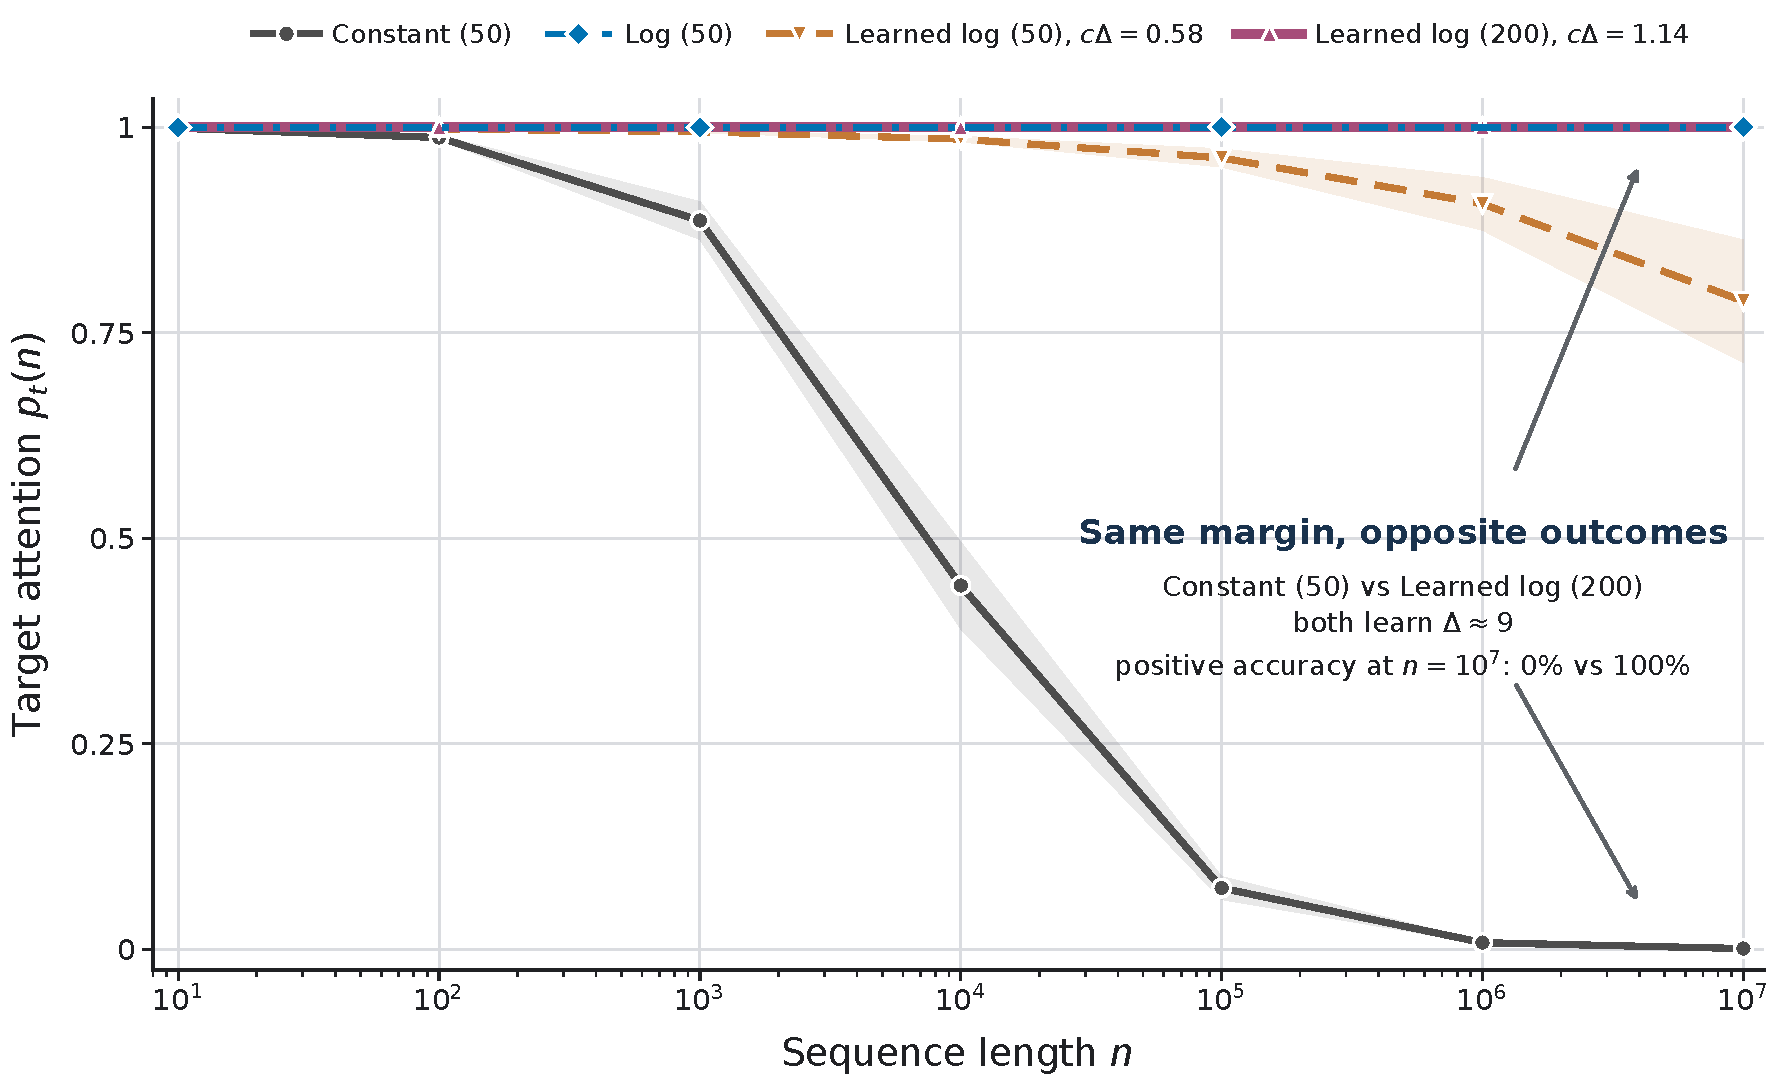
\includegraphics[width=18.50in]{../figures/poster_target_attention_by_length.pdf}
\end{center}

\vfill
\begin{center}
{\SmallFont\color{Muted}
Means over five seeds; bands show $\pm1$ s.d.}
\end{center}
\end{minipage}
\end{contentcard}
\end{minipage}%
\hspace{0.45in}%
\begin{minipage}[t]{9.30in}
\vspace{0pt}
\begin{contentcard}[height=12.40in]
\sectionheading{Learned-Log Threshold}
\begin{center}
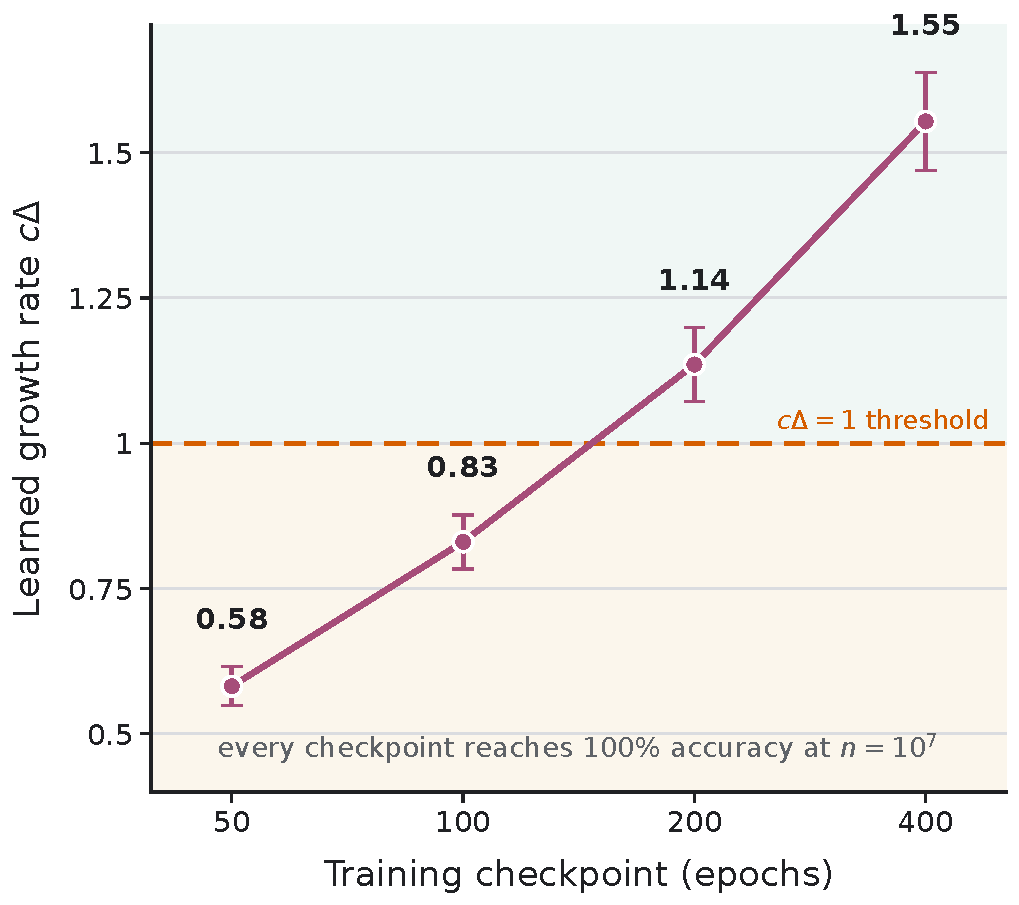
\includegraphics[width=8.50in]{../figures/poster_learned_log_threshold.pdf}
\end{center}

\begin{center}
{\SmallFont\color{Muted}
Means over five seeds; error bars show $\pm1$ s.d.}
\end{center}

\begin{insightbox}
\SmallFont
\textbf{A Finite Pass Can Hide Later Failure.} Checkpoints below $c\Delta=1$
pass the $n=10^7$ benchmark yet are predicted to fail at greater lengths.
\end{insightbox}
\end{contentcard}

\vspace{0.28in}
\begin{contentcard}[height=7.20in]
\sectionheading{Key Takeaways \& Scope}
\takeawaynum{1}\hspace{0.10in}\textbf{Fixed scaling postpones, but cannot
prevent, target-attention dilution.}

\vspace{0.10in}
\takeawaynum{2}\hspace{0.10in}\textbf{Sufficiently strong logarithmic
sharpening can prevent dilution.}

{\SmallFont Target attention converges to one when $\Delta>1$ (Log) or
$c\Delta>1$ (Learned log).}

\begin{scopebox}
\SmallFont
\textbf{Scope.} These thresholds are exact for the reduced two-score classifier
studied here; whether analogous conditions hold in full transformers remains
open.
\end{scopebox}
\end{contentcard}

\vspace{0.28in}
\begin{contentcard}[height=4.64in]
\sectionheading{References \& Acknowledgments}
\TinyFont
\textbf{[1]} Vaswani et al. (2017). \textit{Attention Is All You Need.}
NeurIPS.\par
\textbf{[2]} Press et al. (2022). \textit{Train Short, Test Long: Attention
with Linear Biases Enables Input Length Extrapolation.} ICLR.

\vspace{0.10in}
\textbf{Acknowledgments.} I thank Professor MacCormick for proposing the
reduced-model direction and for guidance on the scope and presentation of this
work.
\end{contentcard}
\end{minipage}

\end{document}
